%Zeigerdiagramme


\begin{frame}
    \fta{Grundlagen Komplexe Zahlen}

     
    \s{
        Die in der Wechselstromtechnik genutzen Zeigerdiagramme geben einen schnellen Überblich über die Größe und
        die Ausrichtung der Spannung und des Stromes. Die zugrunde liegenden Begriffe der komplexen Zahlenebene und
        der Aufbau von Zeigerdiagrammen wird folgend weiter Erläutert und an einem Beispiel erklärt.
    }



    \begin{Lernziele}{Komplexe Zahlen}
        Die Studierenden können
        \begin{itemize}
            \item mit Zahlen in der komplexen Ebene umgehen.
            \item Zeigerdiagramme von komplexen Zahlen darstellen.
            \item komplexe Zahlen berechnen.
        \end{itemize}
    \end{Lernziele}

\end{frame}

\begin{frame}
    \ftb{Komplexe Zahlenebene}

    \s{
        Um den Aufbau von Zeigerdiagrammen zu Überblicken ist ein grundlegendes Verständnis über die komplexe 
        Zahlenebene nötig. Für die elementaren Rechenoperationen reichen die natürlichen Zahlen mit Null und die 
        rationalen Zahlen aus. Die rationalen Zahlen können als endliche oder periodische Dezimalzahlen dargestellt 
        werden. Die irrationalen Zahlen lassen sich hingegen als Dezimalzahlen darstellen, welche unendliche viele
        Stellen aufweisen und dabei nicht periodisch sind. Die reellen Zahlen setzen sich aus den rationalen Zahlen
        und den irrationalen Zahlen zusammen. Allerdings ist beispielsweise das Wurzelziehen aus einer negativen Zahl 
        in der reellen Zahlenebene nicht möglich. Hierfür wird die komplexe Zahlenebene eingeführt. in der komplexen 
        Zahlenebene wird der Raum der reellen Zahlen um die imaginäre Einheit j erweitert. So ergibt in der komplexen
        Zahlenebene das Wurzelziehen aus -1 die imaginäre Einheit j. 
    }

    \b{
        In der komplexen Zahlenebene wird die imaginäre Einheit j eingeführt, um mit komplexen Zahlen zu rechnen.
    }

    \begin{eq}
        \mathrm{j}=\sqrt{-1} 
    \end{eq}

        Das Quadrieren der imaginären Einheit ergibt wiederum -1. 
    
    \begin{eq}
        \mathrm{j}^2=-1
    \end{eq}
\end{frame}


\begin{frame}
    \ftx{Darstellung von komplexen Zahlen}

    \s{
        Eine komplexe Zahl \underline{Z} beschreibt einen Ort in der komplexen Ebene. Um in einem zweidimensionalen
        Koordinatensystem einen Ort eindeutig festzulegen werden zwei Koordinaten benötigt. Die beiden Koordinaten zur 
        Beschreibung einer komplexen Zahl \underline{Z} werden in der komplexen Ebene als Realteil und Imaginärteil 
        beschrieben (vgl. Gleichung \ref{GleichungKomplexeZahlen}). Komplexe Zahlen werden meist durch einen Unterstrich 
        gekennzeichnet, wobei der Realteil und der Imaginärteil reelle Zahlen darstellen. 
    }

    \b{
        Kartesische Koordinaten mit dem Realteil und dem Podukt aus imaginärer Einheit und Imaginärteil:
    }

    \begin{eq}
        \underline{Z}=Realteil+\mathrm{j} \cdot Imagin"arteil  \label{GleichungKomplexeZahlen}
    \end{eq}
    \begin{eq}
        \underline{Z}=\Re(\underline{Z})+\mathrm{j} \cdot \Im(\underline{Z})  
    \end{eq}

\end{frame}


\begin{frame}
    \ftx{Darstellung von komplexen Zahlen}

    \s{
        In der Komplexene Ebene wird der Realteil auf die Abzisse und der Imaginärteil auf die Ordinate aufgetragen. 
        Es werden die Abkürzungen Re = Realteil und Im = Imaginärteil verwendet. Das Koordinatensystem einer komplexen 
        Ebene wird in der Abbildung \ref{BildKomplexeEbene} erläutert. Der Ort der komplexen Zahl kann durch 
        Richtungspfeile, welche auch als Vektoren oder Zeiger bezeichnet werden, dargestellt werden. Die Darstellung
        der komplexen Zahl in kartesischen Koordinaten erfolgt durch die Zerlegung in Realteil der komplexen Zahl 
        Re(\underline{Z}) und Imaginärteil der komplexen Zahl Im(\underline{Z}) kombiniert mit der imaginären Einheit j. 
        Komplexe Zahlen können auch in Polar-Koordinaten dargestellt werden. Dies erfolgt durch den Betrag $|\underline{Z}|$
        der komplexen Zahl \underline{Z} und durch den Winkel $\varphi$, den der Zeiger der komplexen Zahl mit der reellen Achse 
        einschließt. 
    }

    \b{
        Verwendung der komplexenen Ebene:
        \begin{itemize}
            \item<1-> Der Realteil $\Re$ wird auf der vertikalen und der Imaginärteil $\Im$ auf der horizontalen Achse aufgetragen
            \item<2-> Kartesische Koordinaten: $\Re(\underline{Z}) + \mathrm{j} \cdot \Im(\underline{Z})$
            \item<3-> Polar-Koordinaten: $|\underline{Z}| \cdot e^{j \cdot \varphi_\mathrm{Z}}  $
        \end{itemize}
    }

    \fu{
        \begin{tikzpicture}
    \draw (0,0) coordinate (K);
    \draw[very thin,color=gray] (-0.1,-0.1) grid (4.2,3.1);
    \draw[->] (-0.2,0) -- (4.4,0) node[right] {$\Re$};
    \draw[->] (0,-0.1) -- (0,3.2) node[above] {$\Im$};
    \pause
    \draw[->, color=blue] (0,0.02) -- (3,0.02) coordinate (R);
    \draw[color = blue] (3,0)node[below]	 {$\Re(\underline{Z})$};
    \draw[->, color=red] (3,0.02) -- (3,2.02) coordinate (Z);
    \draw[color = red] (3,1)node[right]	 {$\Im(\underline{Z})$};
    \draw[->] (0,0.02) -- (3,2.02);
    \draw(2.3,1.9) node	 {$\underline{Z}$};
    \pause

    %Winkel
    \draw pic[draw, angle radius = 1.2cm, <-] {angle = R--K--Z};
    \draw(1.4,0.5) node{$\varphi_\mathrm{Z}$};
    \draw(1,1)node {$|\underline{Z}|$};
\end{tikzpicture}
    }{{\bf Zeigerdiagramm einer komplexen Zahl.} Eine komplexe Zahl $\underline{Z}$, welche sich durch $Re(\underline{Z})$ und $Im(\underline{Z})$
    in kartesischen Koordinaten und durch den Betrag der komplexen Zahl $|\underline{Z}|$ sowie den zugehörigen Winkel
    $\varphi$ in Polar-Kooradinaten darstellen lässt. \label{BildKomplexeEbene}}

\end{frame}


\begin{frame}
    \ftx{Koordinatentransformation}

    \s{
        Die beiden Darstellungsformen lassen sich ineinander transformieren. Behilflich ist hier die Euler'sche Formel. 
        Die Euler'sche Formel zeigt, dass sich der Ordinatenwert und der Abzissenwert des Einheitskreises
        durch die trigonometrischen Funktionen Kosinus und Sinus berechnen lassen. Die Euler'sche Formel wird in der Gleichung 
        \ref{GleichungEuler} dargestellt. 

        \begin{eq}
            \mathrm{e}^{\mathrm{j} \cdot \chi} = \cos(\chi) + \mathrm{j} \cdot \sin(\chi)    \label{GleichungEuler}
        \end{eq}
    
        Unter Verwendung der Euler'schen Formel können durch die Hinzunahme des Betrages der komplexen Zahl die Polar-Koordinaten
        in kartesische Koordinaten transformiert werden. Dies wird durch die Gleichung \ref{GleichungKartesisch} erläutert. 
    
        \begin{eq}
            \underline{Z} = |\underline{Z}| \cdot \cos(\varphi) + \mathrm{j} \cdot |\underline{Z}| \cdot \sin(\varphi) = \Re(\underline{Z}) + \mathrm{j} \cdot \Im(\underline{Z}) \label{GleichungKartesisch}
        \end{eq}
    
        Über den Satz des Pythagoras lässt sich aus den bekannten Realteil und Imaginärteil der Betrag der komplexen Zahl
        für die Polar-Koordianten bestimmen. Der dazugehörige Winkel ergibt sich aus dem arctan mit dem Verhältnis aus Imaginärteil
        zu Realteil im Argument. Mit diesen Informationen kann eine komplexe Zahl wie in der Gleichung \ref{GleichungPolar} 
        in Polar-Koordinaten transformiert werden. 
    
        \begin{eq}
            \underline{Z} = \sqrt{(\Re(\underline{Z}))^2+(\Im(\underline{Z}))^2} \cdot \mathrm{e}^{\mathrm{j} \cdot \arctan(\frac{\Im(\underline{Z})}{\Re(\underline{Z})}) } = |\underline{Z}| \cdot \mathrm{e}^{\mathrm{j} \cdot \varphi} \label{GleichungPolar}
        \end{eq}
    }

    \b{
        \begin{itemize}
            \item Euler'sche Formel: 
            \begin{eq}
                \mathrm{e}^{\mathrm{j} \cdot \chi} = \cos(\chi) + \mathrm{j} \cdot \sin(\chi)  
            \end{eq}
            \item Kartesische Koordianten:
            \begin{eq}
                \underline{Z} = |\underline{Z}| \cdot \cos(\varphi) + \mathrm{j} \cdot |\underline{Z}| \cdot \sin(\varphi) = \Re(\underline{Z}) + \mathrm{j} \cdot \Im(\underline{Z}) 
            \end{eq}
            \item Polar-Koordinaten:
            \begin{eq}
                \underline{Z} = \sqrt{(\Re(\underline{Z}))^2+(\Im(\underline{Z}))^2} \cdot \mathrm{e}^{\mathrm{j} \cdot \arctan(\frac{\Im(\underline{Z})}{\Re(\underline{Z})}) } = |\underline{Z}| \cdot e^{j \cdot \varphi} 
            \end{eq}
        \end{itemize}
    }
\end{frame}


\begin{frame}
    \ftx{Darstellungsformen komplexer Zahlen}

    \begin{Merksatz}{Darstellungsformen komplexer Zahlen}
        Kartesische Darstellung:
        \begin{eq}
            \underline{Z} = \Re(\underline{Z}) + j \cdot \Im(\underline{Z}) \nonumber
        \end{eq}
        Polarform:
        \begin{eq}
            \underline{Z} = |\underline{Z}| \cdot e^{j \cdot \varphi}   \nonumber
        \end{eq}
        Trigonometrische Darstellung:
        \begin{eq}
            \underline{Z} = |\underline{Z}| (\cos(\varphi) + j \cdot \sin(\varphi))   \nonumber
        \end{eq}
    \end{Merksatz}

\end{frame}

\begin{frame}
    \ftx{Grundrechenarten und Operationen}

    \s{
        Zu den Operationen bei komplexen Zahlen zählt die Konjugation. Beim Konjugieren einer komplexen Zahl wird der 
        j durch -j ersetzt (Negation des Imaginärteils). Die Konjugation wird wie in Gleichung \ref{GleichungKonj} dargestellt mit einem
        Stern gekennzeichnet. 
    }

    \b{
        Konjugation:
    }

    \begin{eq}
        \underline{Z}^* = (\Re(\underline{Z}) + \mathrm{j} \cdot \Im(\underline{Z}))^*= \Re(\underline{Z}) - \mathrm{j} \cdot \Im(\underline{Z})   \label{GleichungKonj}
    \end{eq}

    \s{
        Der Betrag einer komplexen Zahl lässt sich durch die Multiplikation der komplexen Zahl mit ihrer Konjugierten
        bestimmen (vgl. Gleichung \ref{GleichungBetrag}). Statt des Betrages, welcher eine Wurzel enthält, wird auch das Betragsquadrat 
        verwendet. Es stellt ebenfalls ein Maß für den Abstand der Zahl zum Ursprung dar, ist aber einfacher zu berechnen.
    }

    \b{
        Betrag und Betragsquadtrat
    }

    \begin{eq}
        |\underline{Z}| = \sqrt{\underline{Z} \cdot \underline{Z}^*} \rightarrow |\underline{Z}|^2 = \underline{Z} \cdot \underline{Z}^*        \label{GleichungBetrag}
    \end{eq}
\end{frame}

\begin{frame}
    \ftx{Grundrechenarten und Operationen}
    \s{
        Bei der Addition und der Subtraktion von komplexen Zahlen empfiehlt es sich, diese zunächst in kartesiche 
        Koordianten umzuwandeln. Auf diese Weise lassen sich der Realteil und der Imaginärteil der komplexen Zahl
        separat miteinander verrechnen. 
    }
    \b{
        Addition und Subtraktion:
    }
    \begin{eqa}
        \underline{Z}_1+\underline{Z}_2 = \Re(\underline{Z}_1) + \Re(\underline{Z}_2) +j \cdot (\Im(\underline{Z}_1) + \Im(\underline{Z}_2)) \\
        \underline{Z}_1-\underline{Z}_2 = \Re(\underline{Z}_1) - \Re(\underline{Z}_2) -j \cdot (\Im(\underline{Z}_1) - \Im(\underline{Z}_2))
    \end{eqa}

    \s{
        Die Darstellung in Polar-Koordinaten empfiehlt sich für die Verrechnungen von komplexen Zahlen durch Multiplikation
        und Division. Die Multiplikation von komplexen Zahlen setzt sich auf dem Produkt der Beträge und der Summe der jeweiligen
        Winkel zusammen (vgl. Gleichung \ref{GleichungMultiplikation}). Bei der Division werden die Beträge dividiert und die Winkel 
        voneinander subtrahiert (vgl. Gleichung \ref{GleichungDivision}). 
    }

    \b{
        Multiplikation und Division:
    }

    \begin{eq}
        \underline{Z}_1 \cdot \underline{Z}_2 = |\underline{Z}_1| \cdot |\underline{Z}_2| \cdot e^{j \cdot (\varphi_1+\varphi_2)} \label{GleichungMultiplikation}
    \end{eq}

    \begin{eq}
        \frac{\underline{Z}_1}{\underline{Z}_2} = \frac{|\underline{Z}_1|}{|\underline{Z}_2|} \cdot e^{j \cdot (\varphi_1-\varphi_2)} \label{GleichungDivision}
    \end{eq}
\end{frame}


\begin{frame}
    \ftx{Grundrechenarten komplexer Zahlen}

    \begin{Merksatz}{Grundrechenarten komplexer Zahlen}
        Für die {\bf Addition und Subtraktion} wird in der Regel die {\bf kartesische Darstellungsform} für komplexen Zahlen verwendet.
        Bei der {\bf Multiplikation und Division} von komplexen Zahlen wird die {\bf Polarform} gewählt. 
    \end{Merksatz}

\end{frame}


\begin{frame}
    \ftx{Grundrechenarten und Operationen}
    \s{
        Da die Division zunächst nur für reelle Zahlen außer Null definiert ist, wird die komplexe Zahl im Nenner so erweitert, dass 
        dieser reell wird.
    }
    \b{
        Division durch konjugiert komplexe Erweiterung:
    }
    \begin{eq}
        \frac{\underline{Z}_1}{\underline{Z}_2} = \frac{\underline{Z}_1}{\underline{Z}_2} \cdot \frac{\underline{Z}_2^*}{\underline{Z}_2^*} = \frac{\underline{Z}_1 \cdot \underline{Z}_2^*}{|\underline{Z}_2|^*} 
    \end{eq}

    \s{
        Durch die Addition einer komplexen Zahl mit ihrer konjugiert komplexen hebt sich ihr Imaginärteil auf (vgl. Gleichung \ref{GleichungRealteil}). 
        Entsprechend verschwindet durch die Subtraktion der Realteil (vgl. Gleichung \ref{GleichungImaginärteil}).
    }
    \b{
        Realteil und Imaginärteil berechnen:
    }
    \begin{eq}
        \Re(\underline{Z}) = \frac{\underline{Z}+\underline{Z}^*}{2} \label{GleichungRealteil}
    \end{eq}
    \begin{eq}    
        \Im(\underline{Z}) = \frac{\underline{Z}-\underline{Z}^*}{2j} \label{GleichungImaginärteil}
    \end{eq}
\end{frame}


\begin{frame}
    \ftb{Graphische Darstellung und Rechnungen mit komplexen Zahlen}

    \s{
        Mithilfe von Zeigerdiagrammen lassen sich komplexe Zahlen auch zeichnerisch lösen. Werden die komplexen
        Zahlen wie empfohlen in der kartesischen Form dargestellt, können die Bestandteile der Realteile und der 
        Imaginärteile direkt abgelesen werden und in ein Koordinatensystem eingestragen werden. Die komplexen Zahlen 
        werden beispielsweise in der Abbildung X eingetragenen. Bei der Addition von komplexen Zahlen wird entweder
        $Z_\mathrm{1}$ an $Z_\mathrm{2}$ gesetzt oder umgekehrt. Denn bei der Addition gilt weiterhin das Kommutativgesetz. Hier werden durch 
        die gestrichelten Pfeile die Parallelverschiebungen von $Z_\mathrm{1}$ und $Z_\mathrm{2}$ angegeben. Die Verschiebungen enden beide an 
        der selben Koordinate. Hier können separat der Realteil und der Imaginärteil aus der Summe der beiden komplexen 
        Zahlen abgelesen werden. 
    }

    \b{
        Rechenoperationen im Zeigerdiagramm - Addition:

        \begin{itemize}
            \item[1.] <2-> Parallelverschiebung $Z_\mathrm{2}$ an die Spitze von $Z_\mathrm{1}$
            \item[2.] <3-> Realteil und Imaginärteil ablesen
        \end{itemize}
    }

    \fu{
        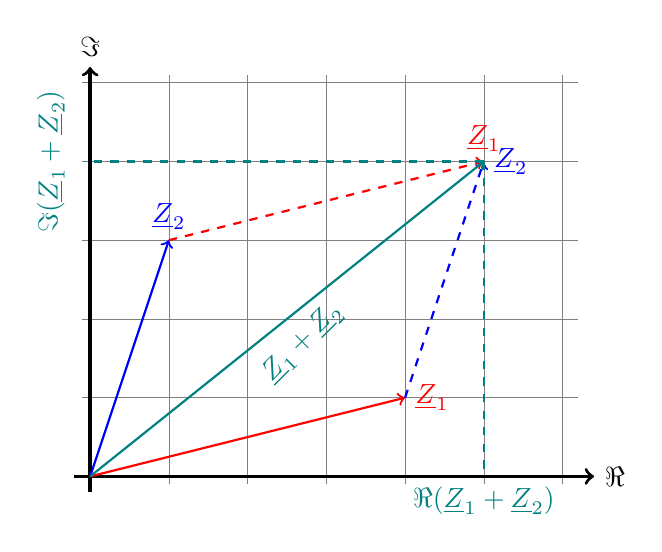
\begin{tikzpicture}
    \draw (0,0) coordinate (K);
    \draw[very thin,gray] (-0.1,-0.1) grid (6.2,5.1);
    \draw[->, very thick] (-0.2,0) -- (6.4,0) node[right] {$\Re$};
    \draw[->, very thick] (0,-0.2) -- (0,5.2) node[above] {$\Im$};
    \draw[->, thick, red] (0,0) -- (4,1) node[right] {$\underline{Z}_\mathrm{1}$};
    \draw[->, thick, blue] (0,0) -- (1,3) node[above] {$\underline{Z}_\mathrm{2}$};
    \pause

    \draw[->, dashed, thick, blue] (4,1) -- (5,4) node[right] {$\underline{Z}_\mathrm{2}$};
    \draw[->, dashed, thick, red] (1,3) -- (5,4) node[above] {$\underline{Z}_\mathrm{1}$};
    \pause

    \draw[->, thick, teal] (0,0) -- (5,4);
    \draw(2.7,1.7) node [teal, rotate=45] {$\underline{Z}_\mathrm{1}+\underline{Z}_\mathrm{2}$};
    \draw[dashed, thick, teal] (5,4) -- (0,4)
    (-0.5,4) node[rotate=90] {$\Im(\underline{Z}_\mathrm{1}+\underline{Z}_\mathrm{2}$)};
    \draw[dashed, thick, teal] (5,4) -- (5,0) node[below] {$\Re(\underline{Z}_\mathrm{1}+\underline{Z}_\mathrm{2}$)};
\end{tikzpicture}
    }{{\bf Addition von komplexen Zahlen.} Zeichnerische Lösung einer Addition von zwei komplexen Zahlen im Zeigerdiagramm}
\end{frame}


\begin{frame}
    \ftx{Zeigerdiagramme - Subtraktion}

    \s{
        Die zeichnerische Lösung der Subtraktion von komplexen Zahlen erfolgt vergleichbar mit der Addition. 
        Zu beachten ist dabei, dass wie in anderen Zahlensystemen bei der Subtraktion von zwei komplexen Zahlen
        das Kommutativgesetz nicht gilt. Wird von der komplexen Zahl $Z_\mathrm{2}$ $Z_\mathrm{1}$ subtrahiert, ändert sich die Richtung
        von $Z_\mathrm{1}$. Hier erfolgt dann wieder die Parallelverschiebung, allerdings lediglich von $Z_\mathrm{1}$. An dem sich ergebenen
        neuen Vektor können dann wieder der Realteil und der Imaginärteil abgelesenw erden. 
    }

    \b{
        Rechenoperationen im Zeigerdiagramm - Subtraktion:

        \begin{itemize}
            \item[1.] <1-> Zeigerumkehr bei Negation
            \item[2.] <2-> Zeiger $Z_\mathrm{1}$ verschieben: Fußpunkt von $Z_\mathrm{1}$ zur Spitze von $Z_\mathrm{2}$
            \item[3.] <3-> Realteil und Imaginärteil ablesen
        \end{itemize}
    }

    \fu{
        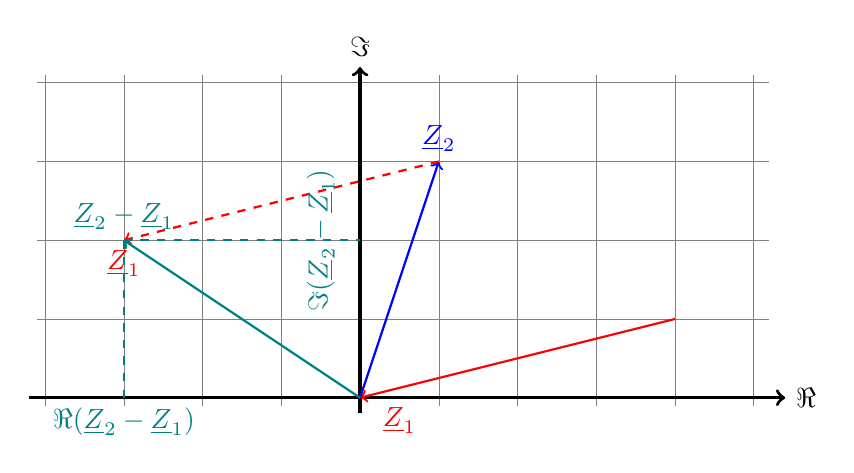
\begin{tikzpicture}
    \draw (0,0) coordinate (K);
    \draw[very thin,gray] (-4.1,-0.1) grid (5.2,4.1);
    \draw[->, very thick] (-4.2,0) -- (5.4,0) node[right] {$\Re$};
    \draw[->, very thick] (0,-0.2) -- (0,4.2) node[above] {$\Im$};
    \draw[->, thick, red] (4,1) -- (0,0);
    \draw(0.5,0) node [below,red] {$\underline{Z}_\mathrm{1}$};
    \draw[->, thick, blue] (0,0) -- (1,3) node[above] {$\underline{Z}_\mathrm{2}$};
    \pause

    \draw[->, dashed, thick, red] (1,3) -- (-3,2) node[left, below] {$\underline{Z}_\mathrm{1}$};
    \pause

    \draw[->, thick, teal] (0,0) -- (-3,2) node [teal, above] {$\underline{Z}_\mathrm{2}-\underline{Z}_\mathrm{1}$};
    \draw[dashed, thick, teal] (-3,2) -- (0,2)
    (-0.5,2) node[rotate=90] {$\Im(\underline{Z}_\mathrm{2}-\underline{Z}_\mathrm{1}$)};
    \draw[dashed, thick, teal] (-3,2) -- (-3,0) node[below] {$\Re(\underline{Z}_\mathrm{2}-\underline{Z}_\mathrm{1}$)};
\end{tikzpicture}
    }{{\bf Subtraktion von komplexen Zahlen.} Zeichnerische Lösung einer Subtraktion von zwei komplexen Zahlen im Zeigerdiagramm}
\end{frame}

  
\begin{frame}
    \ftx{Zeigerdiagramme - Multiplikation}

    \s{
        Die in der Abbildung \ref{BildMultiplikation} dargestellten komplexen Zahlen $\underline{Z}_\mathrm{1}$ und $\underline{Z}_\mathrm{2}$ werden zur 
        Multiplikation in Polar-Koordinaten abgebildet. Durch die zuvor beschriebenen Rechnenregeln der Multiplikation 
        für komplexe Zahlen können die Werte für die für das Ergebnis $\underline{Z}_\mathrm{3}$ bestimmt werden. Die Multiplikation
        aus den Zeigerlängen gibt die Länge des Produktes an. Die Summe aus den beiden komplexen Zahlen den Winkel der neuen
        komplexen Zahl an. 
    }

    \b{
        Rechenoperationen im Zeigerdiagramm - Multiplikation: (Zeichnung nicht maßstabsgetreu!)

        \begin{itemize}
            \item[1.] <2-> Winkel $\varphi_\mathrm{1}+\varphi_\mathrm{2}$ berechnen und einzeichnen
            \item[2.] <3-> Länge $Z_1 \cdot Z_\mathrm{2}$ berechnen und eintragen
            \item[3.] <4-> Realteil und Imaginärteil ablesen
        \end{itemize}
    }
    
    \fu{
        \begin{tikzpicture}
    \draw (0,0) coordinate (U);
    \draw (4,0) coordinate (0);
    \draw[very thin,gray] (-3.1,-0.1) grid (5.2,4.1);
    \draw[->, very thick] (-3.2,0) -- (5.4,0) node[right] {$\Re$};
    \draw[->, very thick] (0,-0.2) -- (0,4.2) node[above] {$\Im$};
    \draw[->, thick, red] (0,0) -- (4,1) coordinate (1);
    \draw(4,1) node [right,red] {$\underline{Z}_\mathrm{1}$};
    \draw[->, thick, blue] (0,0) -- (1,3) coordinate (2);
    \draw(1,3) node [above,blue] {$\underline{Z}_\mathrm{2}$};
    \draw pic[draw,red, very thick, angle radius = 3cm, ->] {angle = 0--U--1} (3.5,0.5) node[very thick, red]{$\varphi_\mathrm{1}$};
    \draw pic[draw,blue, very thick, angle radius = 2cm, ->] {angle = 0--U--2} (1.5,1.7) node[very thick, blue]{$\varphi_\mathrm{2}$};
    \pause

    \draw (-2,4) coordinate (3);
    \draw pic[draw, teal, very thick, angle radius = 1cm, ->] {angle = 0--U--3} (-1.2,0.5) node[very thick, teal]{$\varphi_\mathrm{1}+\varphi_\mathrm{2}$};
    \pause

    \draw[->, thick, teal] (0,0) -- (-2,4);
    \pause

    \draw[dashed, thick, teal] (-2,0) -- (-2,4) node[above] {$\underline{Z}_\mathrm{2} \cdot \underline{Z}_\mathrm{1}$};
    \draw[dashed, thick, teal] (0,4) -- (-2,4);
\end{tikzpicture}
    }{{\bf Multiplikation von komplexen Zahlen.} Zeichnerische Lösung einer Multiplikation von zwei komplexen Zahlen in Polar-Koordinaten im Zeigerdiagramm. \label{BildMultiplikation}}
\end{frame} 
\newpage